\documentclass[10pt,a4paper,oneside]{book}
\usepackage{amsmath, amssymb, graphicx, hyperref, mathtools}
\graphicspath{{figures/}}

\newcommand{\given}{\;\middle|\;}

\title{A Laboratory Course on Single Molecule Localization Microscopy}

\author{Kyle M. Douglass}

\date{\today}

\begin{document}

\maketitle

\tableofcontents

\chapter{Introduction}

\section{Super-Resolution Fluorescence Microscopy}

Fluorescence microscopy is a set of techniques that allows scientists to study the structure and behavior of microscopic systems. Cell biologists in particular use fluorescence microscopes to visualize biological systems across many different spatial scales, from macromolecular complexes, organelles, and cells to tissues and even whole organisms. The power of fluorescence microscopy comes from the ability to label specific molecules with fluorescent markers such that the presence of light coincides with the presence of the target molecules. This molecular specificity, when combined with a light microscope's ability to magnify specimens that are normally too small to see with the unaided eye, provides a powerful tool to better understand the microscopic world.

All light microscopes, however, are bound by the laws of diffraction which state that the smallest features that can be observed by the instrument are approximately the size of the wavelength of light. Anything smaller than this so-called diffraction limit appears blurred, often to the point where an observer is completely unable to infer its structure from an image. For biologists this is particularly problematic because many important cellular structures have sizes that are smaller than this limit.

Starting in the 1900s researchers began to discover ways to circumvent the diffraction limit of light microscopy and image structures that were smaller than a wavelength with good fidelity. Among the first such techniques that was proposed and realized was the near-field optical microscope, whereby a sample is scanned by an illuminated aperture that is smaller than the wavelength of light. Unfortunately, this technique is somewhat cumbersome to use for cell biology studies because of the constraints that the instrument places on the sample. In the early 1990s it was discovered that the resolution of confocal fluorescence microscopes, a standard instrument in cell biology, could be improved beyond the diffraction limit by up to a factor of two and still remain compatible with biological samples.\footnote{Resolution, as we shall see, is often defined as the smallest distance at which two very small light emitters may be located with respect to one another and still be determined to be separate objects.} Several new techniques quickly followed, such as stimulated emission depletion (STED) microscopy, structured illumination (SIM) microscopy, stochastic optical reconstruction microscopy (STORM)\cite{rust-naturemethods-2006}, and photoactivated localization microscopy (PALM)\cite{betzig-science-2006, hess-biophysicaljournal-2006}. All of these techniques, which collectively would come to be called super-resolution microscopy, were compatible with the requirements of biologists. Additonally, the plethora of techniques present different tradeoffs in terms of spatiotemporal resolutions, signal-to-noise ratios, and live-cell compatibilities so that today's cell biologist can choose the instrument that best suits their needs.

In this course you will learn about a super-resolution fluorescence microscopy technique called \textbf{single molecule localization microscopy}, or SMLM. SMLM uses light to stochasticly manipulate photophysical states of fluorescent molecules such that the images of individual molecules can be located with high precision, often on the order of tens of nanometers. A set of location estimates recorded across time (called localizations), are combined to form an image with a resolution that surpasses the diffraction limit of light. SMLM has been used to study a number of celluar structures and processes, such as the diffusion of membrane proteins, axonal actin rings, the nuclear pore complex, and centrioles.

\section{Learning Outcomes}

\begin{enumerate}
    \item Explain how a modern epifluorescence microscope works, including a list of its main components and their relationships to one another.
    \item Identify the main components of an epifluorescence microscope on the real microscope in the lab.
    \item Explain the principle behind single molecule localization microscopy and how it overcomes the diffraction limit of light.
    \item Model fluorescence phenomena such as photoswitching and photoactivation as continuous-time Markov chains.
    \item Analyze data from the microscope to produce super-resolved images of cellular structures.
\end{enumerate}

\chapter{The Modern Fluorescence Microscope} \label{ch:microscopes}

\section{Epifluorescence Microscopes}

The design of a modern fluorescence microscope is illustrated in \autoref{fig:epifluorescence-microscope}. In this design, light from a source such as a laser or a high intensity LED enters the microscope and is reflected into the objective lens by a dichroic mirror.\footnote{A dichroic mirror is a mirror with an engineered surface that reflects some wavelengths of light and transmits others.} The exictation light is focused by the objective lens onto the sample where it excites fluorescent molecules within the sample. The fluorescence light is collected by the same objective and passes subsequently through the dichroic mirror. A second lens, known as the tube lens, collects the fluorescence light and forms an image of the sample on the camera.

\begin{figure}[ht]
    \centering
    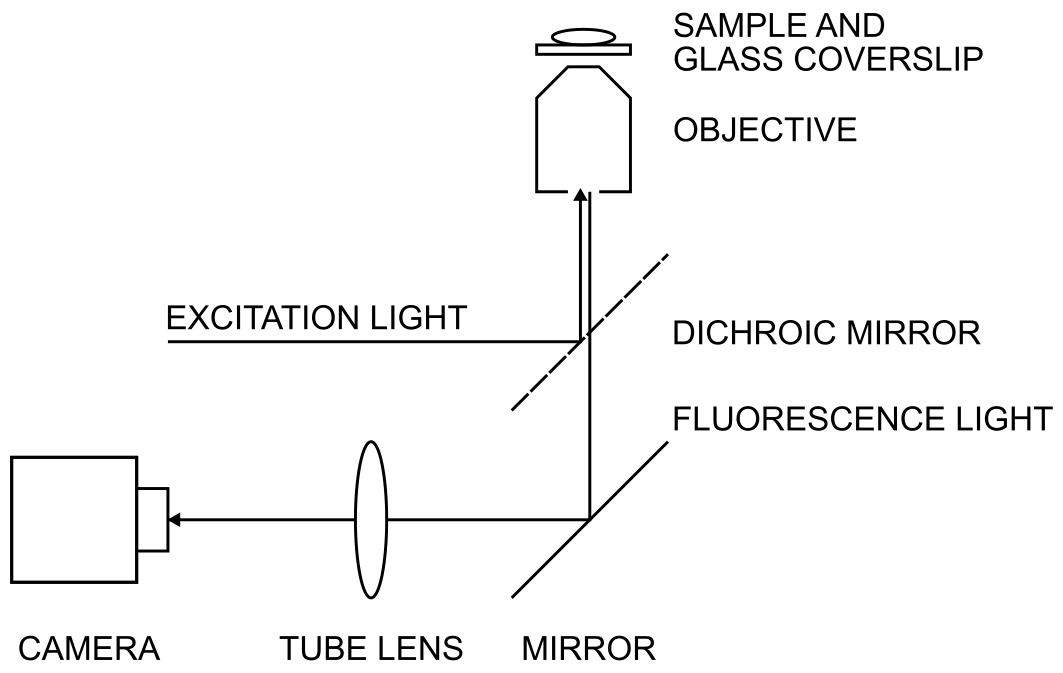
\includegraphics{epifluorescence-microscope.png}
    \caption{Principle components of an infinity corrected epifluorescence microscope.}
    \label{fig:epifluorescence-microscope}
\end{figure}

There are a few important things to understand about this microscope. The first is that the choices for light source, dichroic mirror, and fluorophore are not completely independent.\footnote{This is true for all fluorescence microscopes, not just for the design being discussed here.} The reason for this is largely due to a fluorophore's Stokes shift, or the difference between the excitation light wavelength and the fluorescence wavelength. As a result of this difference, the choice of fluorophore will determine the wavelength of the light source that is necessary. It will also determine the so-called passband of the dichroic mirror; it must be selected so that sufficient amounts of excitation light is reflected and fluorescence light is transmitted. If the dichroic mirror is poorly chosen, either not enough light will illuminate the sample or not enough fluorescence photons will be detected (or both). In practice, the passbands of dichroic mirrors are standardized around a few popular fluorphores, such as green fluorescent protein (GFP).

Another important characteristic of the design illustrated in \autoref{fig:epifluorescence-microscope} is that the sample is excited by the same lens that collects the fluorescence signal. This geometry is known as \textbf{epi-illumination}, as opposed to \textbf{transillumination} whereby the sample is illuminated by light that is focused onto the sample by a separate condenser lens. When imaging fluorescence from a sample and simply reflected light, it is known more specifically as \textbf{epifluorescence}. Epifluorescence microscopes solve the problem of the excitation light dominating the weaker fluorescence signal because most of the excitation light propagates away from the objective after it leaves the sample.

\section{Infinity Corrected Systems}

A final thing to note about the design in \autoref{fig:epifluorescence-microscope} is that the final image of the sample is formed on the camera by a second lens called the tube lens. Modern microscope objectives are infinity corrected. As illustrated in \autoref{fig:infinity-space}, an infinity corrected system places the sample in the front focal plane of the objective lens. The result is that the image of the sample is formed at infinity after the objective and requires the tube lens to form a real image at the camera's sensor plane.

\begin{figure}[ht]
    \centering
    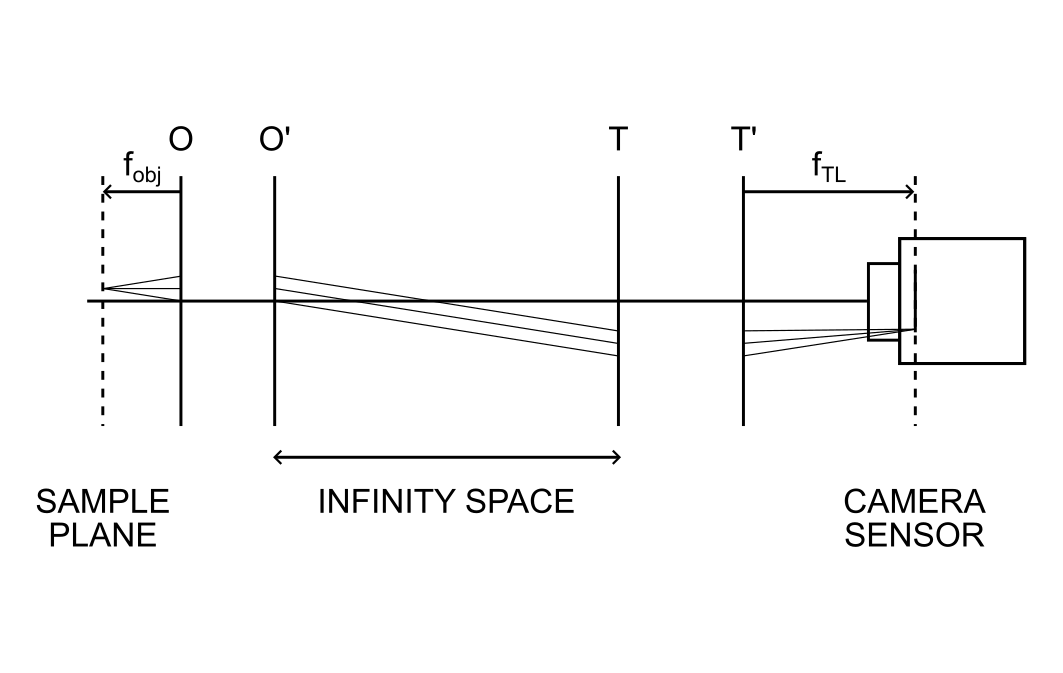
\includegraphics{infinity-space.png}
    \caption{Optical path of an infinity corrected microscope. Rays emitted from a point in the sample plane are parallel in the infinity space. $O/O'$ and $T/T'$ denote the principle planes of the objective and tube lens, respectively. $f_{obj}$ and $f_{TL}$ denote their focal lengths.}
    \label{fig:infinity-space}
\end{figure}

Prior to the development of infinity corrected systems, microscope objectives formed their images at a fixed distance from the objective, called the tube length. By convention, this distance was usually around 160 mm. A second lens, the eye piece, would reform the image for viewing by an observer. Modern microscopy often requires that additonal optical elements be placed after the objective during measurements, such as dichroic mirrors and filters. Upon insertion into the optical path, one of these additonal elements would displace the location of the image formed by a traditional objective due the refractive index difference between the element's material and air. This in turn would force the microscopist to refocus the image and result in a slightly different magnification of the final image. Infinity corrected systems do not suffer from these problems because the intermediate image is located at infinity. As a result, the final image will not change the position when additonal elements are inserted into the so-called infinity space between the objective and tube lens.

\section{Imaging Properties of Microscopes}

\subsection{The Point Spread Function} \label{sec:psf}

One of the most useful tools to characterize the performance of a microscope is the \textbf{point spread function}, or PSF. Qualitatively, the PSF is the image formed by the microscope of an infinitesimally small object emitting light uniformly in all directions. A microscope without aberrations\footnote{An aberration is any deformation of the PSF other than that caused by diffraction.} will have a PSF that is well-modeled by the Airy disk, which is the pattern seen in \autoref{fig:airy-pattern}.

\begin{figure}[ht]
    \centering
    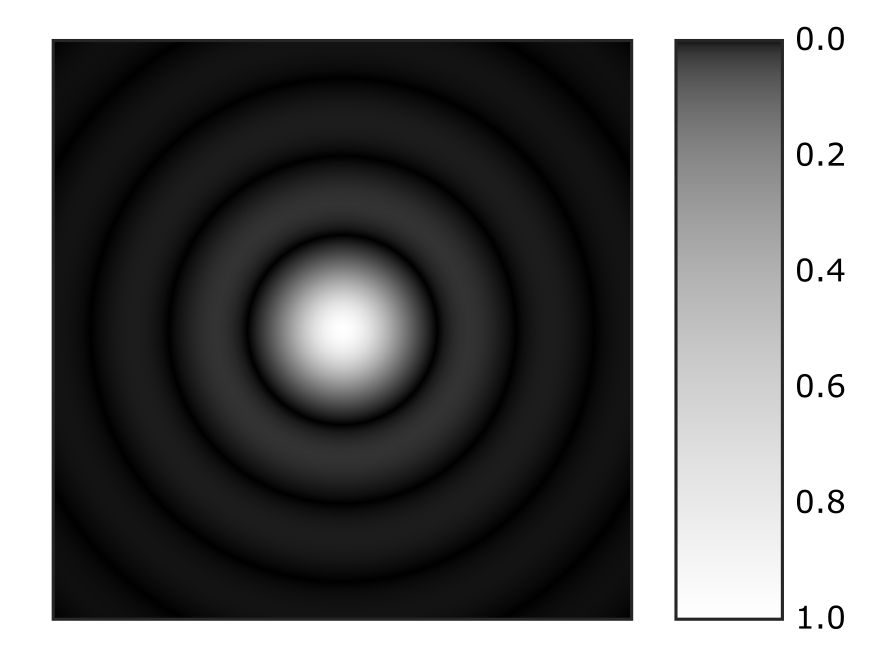
\includegraphics{Airy-pattern.png}
    \caption{The Airy disk pattern. Lighter colors denote regions of higher light intensity. By Sakurambo at English Wikipedia - Public Domain, \url{https://commons.wikimedia.org/w/index.php?curid=18640280}.}
    \label{fig:airy-pattern}
\end{figure}

The expression for the Airy disk is derived from scalar diffraction theory, i.e. the polarization of light is ignored. More precisely, it is the Fraunhofer diffraction pattern of a uniformly-illuminated circular aperture.\footnote{This is identical to solving for the image of an isotropically-emitting, incoherent point source because such a source uniformly fills the system's pupil.} Mathematically, the expression is

\begin{equation}
    I \left(X\right) = I_{0} \left[ \frac{2 J_{1}\left(X\right)}{X} \right]^2
\end{equation}

\noindent where $ X = 2 \pi r \text{NA} / \lambda $, $r$ is the radial coordinate in the image plane, $\text{NA}$ is the numerical aperture of the microscope, and $\lambda$ is the wavelength of light. $J_{1}\left(X\right)$ is called the first-order Bessel function of the first kind. Its first zero, which is important for defining resolution as we shall see later, is at $\Delta X = 3.8317$. In terms of the radial coordinate, it lies at $\Delta r \approx 0.61 \text{NA} / \lambda$.

\subsection{Image Formation in Linear Shift Invariant Systems}

Since the PSF is by definition the image of an infinitesimally small emitter and because it has a finite spatial extent, it follows that the PSF is a measure of the blurring of the image of an object seen through a microscope due to diffraction. But what about samples containing many fluorophores? How does the point spread function affect its image?

We can answer this question if we first assume a few properties about the microscope. The first is linearity, i.e. the image of two fluorophores is just the sum of the image of each fluorophore individually. Fluoresence light emitted from different fluorophores is incoherent, so a fluorescence microscope is linear in the emitted fluorescence intensity.\footnote{A microscope where the object is illuminated by coherent radiation is linear in the electric field.} The second assumption is that the microscope is shift invariant. This means that the PSF does not depend on the location of an emitter. 

Let the density of fluorescence emitters in a plane be represented by $O \left(x, y\right)$. Under the two assumptions above\footnote{These assumptions are equivalent to those used to model linear time invariant systems, which are characterized by an impulse response. The PSF is analogous to the impulse response.}, the resulting image $I \left(x, y\right)$ is the convolution of this density with the PSF, or

\begin{equation} \label{eq:image-formation}
    I \left(x, y\right) = \text{PSF} \left(x, y\right) \ast O \left(x, y\right)
\end{equation}

We can reduce the degree of blurring by increasing the numerical aperture of the objective, which has the effect of reducing the size of the PSF. Ultimately, however, diffraction prevents us from shrinking the PSF down to a point. As a result, a microscope image will never exactly reproduce an image of the object.

\section{Digital Image Formation}

The image described by \autoref{eq:image-formation} is a function of continuous spatial variables $x$ and $y$ and represents the optical power per area at a point $\left(x, y\right)$ in the image plane.\footnote{Equivalently, it is proportional to the photon flux at the image plane in units of $\text{photons} / s / m^2$.} A camera, which is used to record the image, is comprised of regularly-spaced, discrete, photo-sensitive elements called pixels. Each pixel converts the optical signal integrated over the time of exposure into a digital number called an analog-to-digital unit, or ADU. A well-designed camera produces images with pixel values (in units of ADUs) that are proportional to the number of photons that were incident on each pixel during an exposure.

This raises the following question: how many pixels should the PSF span? If the PSF is smaller than a pixel, then we are effectively losing detail in the final image. On the other hand, if the PSF spans many pixels, then we sacrifice signal-to-noise ratio by spreading the photons from a fluorescent molecule out over those pixels. There must be an optimum number of pixels per PSF to balance these two effects.

One approach to the problem is to consider the Nyquist sampling criterion for the entire system. In signal processing, the Nyquist criterion states that we need to sample a signal at twice the rate of its highest frequency component to reconstruct the signal exactly. The equivalent formulation in optics states that we need approximately two pixels per PSF to reconstruct the $I \left(x, y\right)$. For a Gaussian PSF, this analysis leads to a full-width half maximum of 2.355 pixels.

\chapter{Single Molecule Localization Microscopy}

\section{Determination of a Single Molecule's Position}

We saw in \autoref{ch:microscopes} that diffraction determines the size of the smallest object that can be seen through a microscope. This size is approximately equal to half of the wavelength of light, which for visible wavelengths is approximately 250 nm.

Under some conditions, however, we can actually determine the location of single fluorescent molecules to a precision that is roughly 10 times better than the diffraction limit, or on the order of 10 nm. This process is called localizing a molecule, and the resulting estimate of its position is called a localization. The technique to do this is called single molecule localization microscopy, or SMLM.

To understand how SMLM works, let's first consider a sample that consists of a single fluorescent molecule. When excited with light, the molecule emits fluorescence and the microscope will record a blurred image of the molecule. Such an image is shown in \autoref{fig:image-of-single-molecule}. Each pixel in \autoref{fig:image-of-single-molecule} is 160 nm in both the horizontal and vertical directions, which is much greater than the size of the molecule.

\begin{figure}[ht]
    \centering
    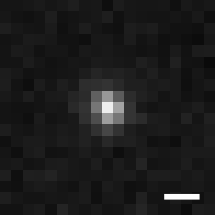
\includegraphics{image-of-single-molecule.png}
    \caption{Image of a single Cy5 fluorescent molecule. Scale bar: 500 nm.}
    \label{fig:image-of-single-molecule}
\end{figure}

The key insight of SMLM is that the position of the molecule is located at the center of its image, and we can find the center to high precision. To do this, we fit a model of the image of a single molecule to the image recorded by the microscope. Two of the model parameters will be the $x$ and $y$ positions of the molecule's center. Thus the result of the fit is an estimate of the molecule's position.

From the discussion in \autoref{sec:psf}, you might think that we need to fit an Airy disk pattern to the image of the fluorophore. In practice, however, this is computationally slow to perform due to the evaluation of the Bessel function. To circumvent this issue, we can use the fact that the Airy disk is approximately the same as a Gaussian function and fit a 2D Gaussian to the image instead. The similarity between the two curves is illustrated in \autoref{fig:airy-vs-gauss}.

\begin{figure}[ht]
    \centering
    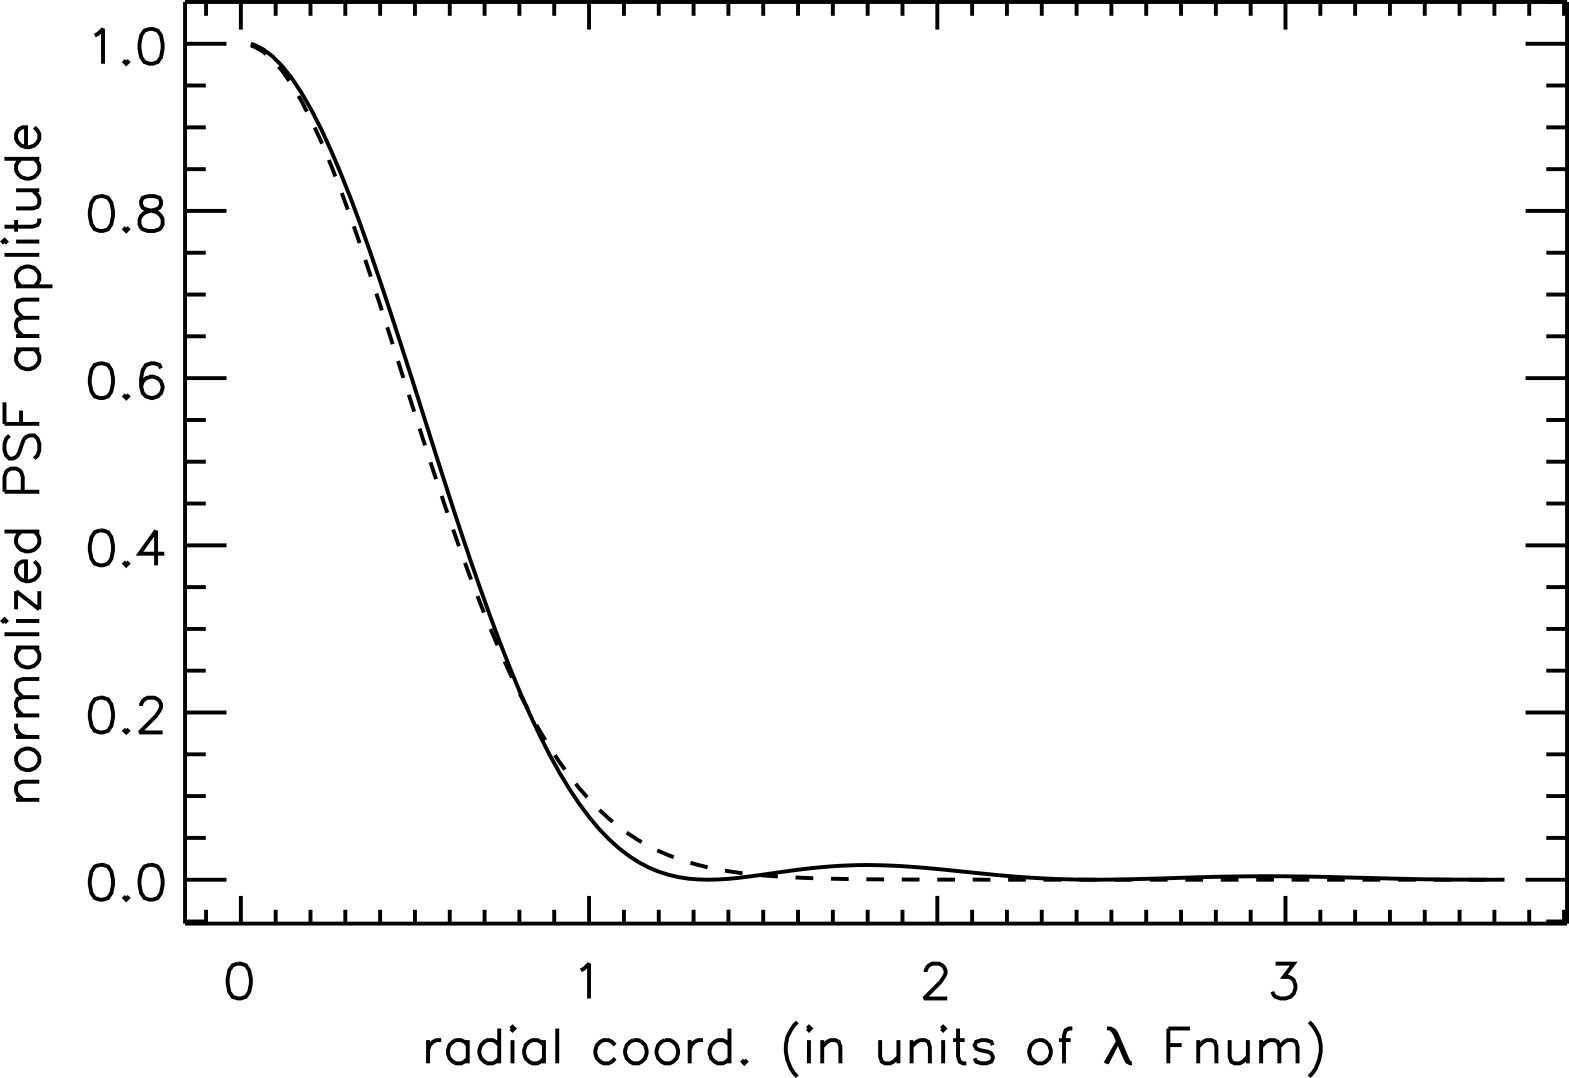
\includegraphics[width=0.75\textwidth]{Airy_vs_gaus.png}
    \caption{Comparison of an Airy disk (solid line) and a Gaussian function (dotted line). By Marius Hagen - Plotted using IDL software., Public Domain, \url{https://commons.wikimedia.org/w/index.php?curid=4230024}.}
    \label{fig:airy-vs-gauss}
\end{figure}

Alternatively, we can fit other models to the image, too. Here are some choices for the model and fit technique that are often used in practice:

\begin{enumerate}
    \item Gaussian least squares fitting
    \item Gaussian maximum likelihood estimation
    \item Phasors
    \item Cubic splines
\end{enumerate}

In practice, the choice of model and fitting technique will involve tradeoffs between speed and precision.

\subsection{Gaussian Least Squares Fitting}

Let $f \left(x, y\right)$ represent the PSF model. A Gaussian model is written as follows:

\begin{equation}
    f \left(x, y\right) = a \exp \left[ \frac{\left(x-x_{0}^2\right) + \left(y - y_{0}^2\right)}{w} \right] + b
\end{equation}

\noindent Here, $x_0$ and $y_0$ represent the center of the molecule in pixels, $w$ is the width of the PSF in pixels, and $a$ and $b$ are related to the maximum pixel signal and the background signal, respectively. Importantly, $x_0$ and $y_0$ are continuous numbers, which means that the center of the molecule may be found with sub-pixel precision.

The position of the molecule is found by minimizing the following objective function using a nonlinear least squares optimizer:

\begin{equation}
    O = \sum_{k=1}^K \left[ s_k - f_{\theta} \left(x_k, y_k\right)\right]^2
\end{equation}

\noindent where there are $K$ pixels with coordinates $\left( x_k, y_k\right)$, and the PSF model parameters are $\theta = \left( x_0, y_0, w, a, b \right)$. Gaussian least squares fitting provides good precision and performance relative to the other techniques.

\subsection{Gaussian Maximum Likelihood Estimation}

This technique also uses a Gaussian PSF model but instead minimizes the following objective function:

\begin{equation}
    \mathcal{L} \left(\theta \given s_1, s_2, \ldots, s_K \right) = \sum_{k=1}^K \left[ s_k \times \ln \left( f_{\theta} \left( x_k, y_k \right) \right) - f_{\theta} \left( x_k, y_k \right) \right]
\end{equation}

\noindent The above equation will contain some additional terms when Gaussian noise from the camera readout is included in the model, but the main idea is there.

The estimates of the PSF parameters $\theta$ from maxmimum likelihood estimation (MLE) are generally more precise than the least squares solution. However, the MLE estimate is slower to compute. You would therefore choose this option if you need better precision but can afford to wait longer for a result.

\subsection{Phasors}

The phasor approach is based on the observation that the first complex coefficients in the horizontal and vertical direction of the discrete Fourier transform of the image contain information on the coordinates of the molecule's position. The angles associated with these coefficients (i.e. the angles of their phasor representations) provide the $x$ and $y$ positions of the molecules.

Unlike the previous two methods, this approach to localizing single molecules is not iterative and is therefore computationally very fast to perform. It is however not as precise as Gaussian fitting.

\subsection{Cubic splines}

The cubic spline approach to single molecule localization involves fitting a 3D cubic spline to PSF data obtained from a calibration routine. This approach is the among the most precise localization methods because the PSF model is interpolated over the measured data, whereas the Gaussian model only assumes a PSF shape. In terms of speed, localizing molecules with cubic splines is relatively slow compared to the other approaches.

\section{Localization Precision}

The estimates of a fluorescent molecule's position have an uncertainty associated with them. This uncertainty is called the localization precision. The localization precison represents the area in which a fluorescent molecule is likely to be located.

There are at least two ways to determine the localization precision in a SMLM experiment. The first is to measure the position of a single molecule multiple times and compute the standard deviation of the resulting distribution of position estimates. The second is to calculate it using the following theoretical formula\cite{thompson-biophysicaljournal-2002}:

\begin{equation}
    \langle \left( \Delta x \right)^2 \rangle = \frac{s^2 + a^{2}/12}{N} + \frac{8 \pi s^4 b^2}{a^2 N^2}
    \label{eq:thompson}
\end{equation}

\noindent In \autoref{eq:thompson}, $\Delta x$ is the squared error in localization, $s$ is the standard deviation of the PSF, $a$ is the size of a pixel, $N$ is the number of photons recorded from the molecule, and $b$ is the number of photons coming from the background. 

The important point to note about \autoref{eq:thompson} is that, in the absence of any background, the localization precision, which is the square root of the above expression, scales as $N^{-1/2}$. This means that improving the number of recorded photons from a molecule by a factor of 100 will improve our estimate of the position by only a factor of 10.

Typically, we can measure between 100 and 10,000 photons from a molecule before it bleaches, and the typical standard deviation of a PSF is around 250 nm. Additonally, the pixel size is often smaller than the size of the PSF. In this case, \ref{eq:thompson} implies that the typical localization precision is then $\Delta x \sim s / N^{1/2}$, or about 25 to 80 nm.

\section{Localizing Dense Distributions of Emitters}

All of the preceding discussion has assumed that we wanted to localize a fluorescent molecule that is well-separated from all others. However, as two fluorescent molecules are brought close together, their images will overlap as illustrated in \autoref{fig:rayleigh}. In this situation, it is impossible to localize them because we don't know how many molecules are present.

\begin{figure}[ht]
    \centering
    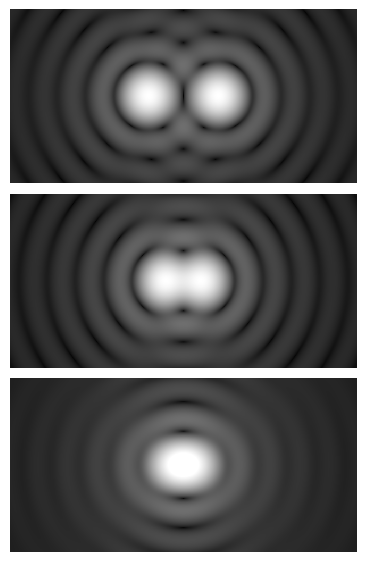
\includegraphics[width=0.6\textwidth]{Airy_disk_spacing_near_Rayleigh_criterion.png}
    \caption{The images of two fluorescent molecules as they are brought close together. They cannot be easily distinguished below a certain distance. Spencer Bliven, Public domain, via Wikimedia Commons. \url{https://commons.wikimedia.org/wiki/File:Airy_disk_spacing_near_Rayleigh_criterion.png}}
    \label{fig:rayleigh}
\end{figure}

This observation poses a severe limitation on applying SMLM to real samples because there will often be a large number of fluorophores within the area spanned by the PSF. The solution to this problem was a significant advance in light microscopy, and was discovered around the same time in the mid 2000's by a few research groups. It helped earn Eric Betzig the Nobel Prize in chemistry in 2014.

To understand how to localize dense distributions of fluorophores, suppose that we could somehow switch on and off the fluorophores. Furthermore, let's imagine that we can do this with enough precision to control which fluorophores are emitting light at any given time. We can localize all the fluorophores in an image if we switch on only a subset of fluorophores where each fluorophore in the subset is separated from all the other fluorophores in the subset by a distance that is greater than the PSF. Then, we can switch off this subset and then switch on a new subset, taking another image. If we repeat this process, we will collect a sequence of images of sparsely distributed, ON-state fluorophores that can be localized. Finally, after localizing all the molecules in all the images we can combine their positions to make a super-resolved image. This process is illustrated \autoref{fig:smlm}. \url{https://www.youtube.com/watch?v=RE70GuMCzww} contains a video demonstrating how the same process can be used to reconstruct an image of the Eiffel from its blinking lights at night.

\begin{figure}
    \centering
    \makebox[\columnwidth][c]{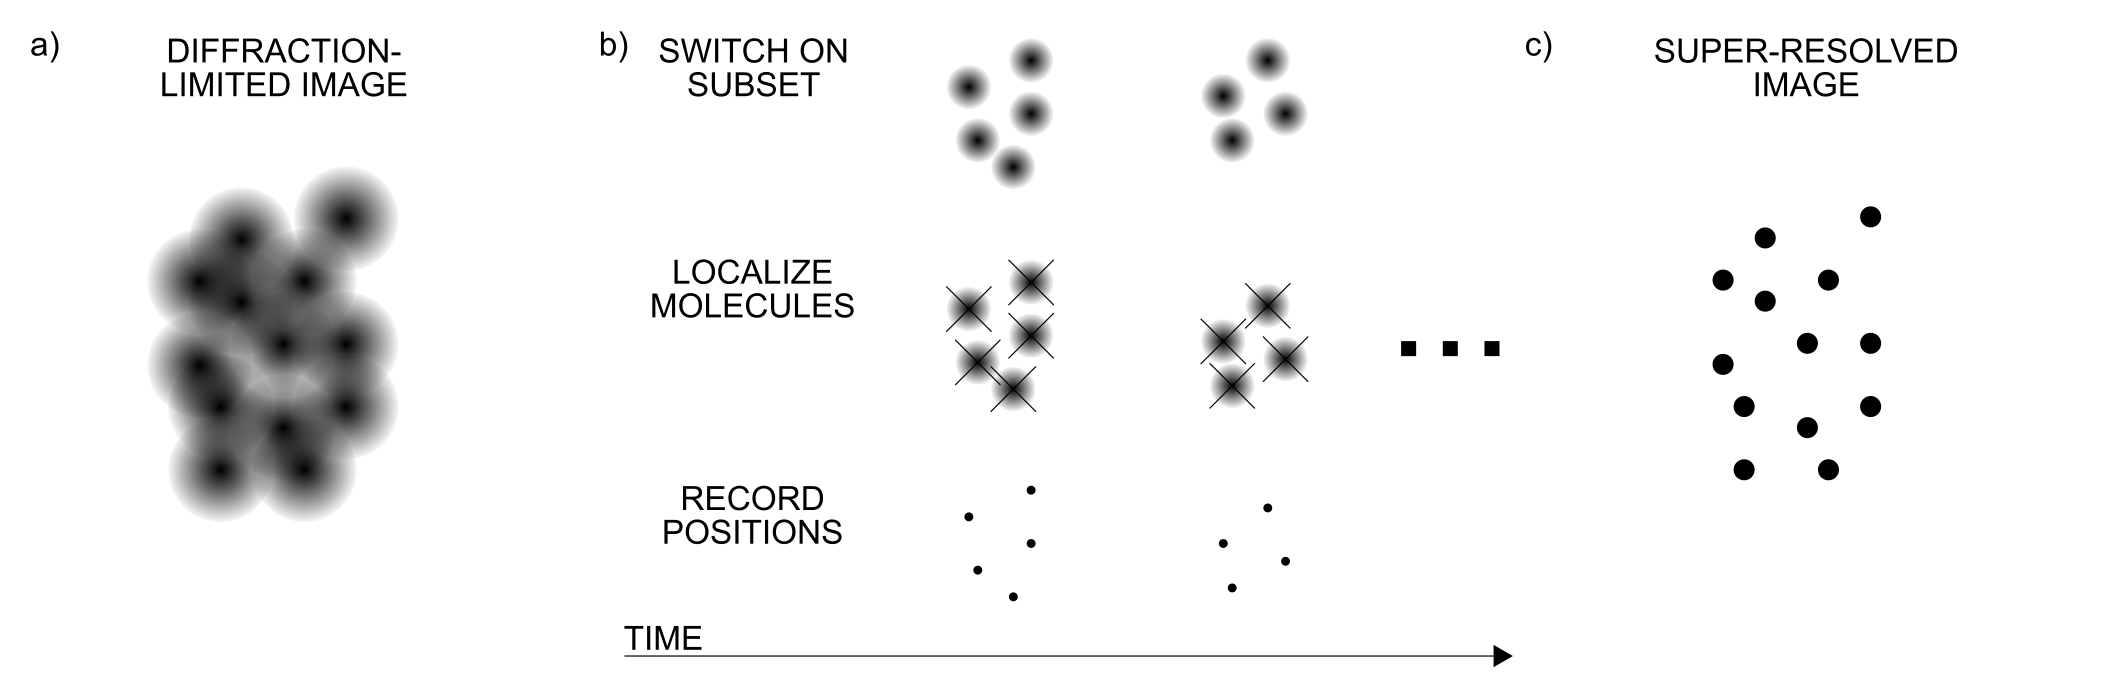
\includegraphics[width=1.3\textwidth]{smlm-principle.png}}%
    \caption{Principle of single molecule localization microscopy. a) A diffraction-limited image from a distribution single fluorophores. Each fluorophore image is a a single point spread function. b) Sequential switching of a sparse subset of fluorophores allows for their localization. c) The final, super-resolved image is reconstructed from the individual localizations.}
    \label{fig:smlm}
\end{figure}

In practice, it takes on the order of ten thousand images to produce a super-resolved image using SMLM, though this order of magnitude can vary depending the structure, the density of fluorescent labels, and more.

We can also infer from \autoref{fig:smlm} that a super-resolved image requires more time to acquire than a simple, diffraction-limited image because we need to acquire many images of different subsets of fluorophores. We can interpret this in terms of a tradeoff between space and time resolutions: to image with higher spatial resolutions we need to sacrifice temporal resolution.

So far we have ignored the mechanism that allows us to switch single fluorophores on and off. This will be discussed in the next chapter.

\chapter{Fluorescence Photophysics}

\section{Energetic States of Fluorophores}

The most important mechanism to achieving super-resolution with SMLM is the ON/OFF switching of fluorophores. Activating only a sparse subset of fluorophores in the ON state at a given time allows us to localize individual fluorophores and, over time, build up a pointilist-like reconstruction of the object.

So, how do we switch on sparse subsets of fluorescent molecules? We take advantage of their photophysical properties, in particular the number of energetic states that the molecule might occupy.

\autoref{fig:alexafluor-energy} illustrates the energy levels in a popular family of fluorophores used in STORM microscopy. Fluorescence occurs when the fluorophore first absorbs a photon and transitions to the excited singlet state $\prescript{1}{}F_1$, then emits a photon of slightly longer wavelength in returning to the singlet ground state $\prescript{1}{}F_0$. After absorbtion by a photon, there is a small chance that the fluorophore will undergo an intersystem crossing ($isc$) to the triplet state $\prescript{3}{}F$. From here, the molecule can react with molecular oxygen to return to the ground singlet state, or react with a thiol that is present in the buffer to form a radical anion, $F^*$. Additionally, the absorption of UV light by the fluorophore in the anion state is higher than in other states, so irradiation by UV light can promote a return to the singlet state.

\begin{figure}[ht]
    \centering
    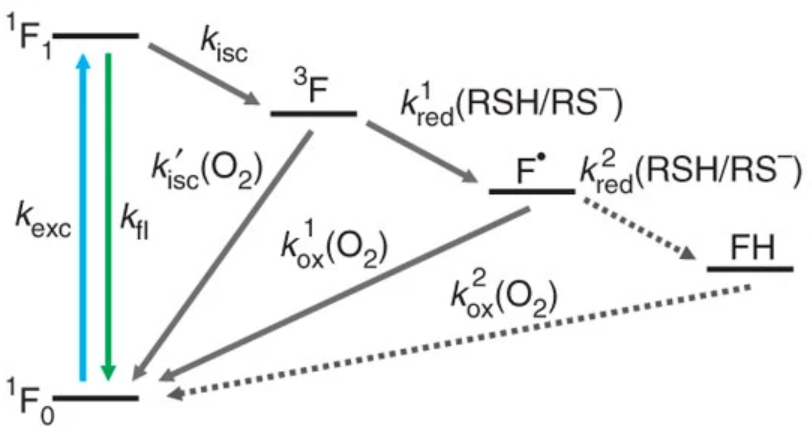
\includegraphics[width=0.8\textwidth]{alexafluor-jablonski-diagram.png}
    \caption{Energy level diagram of flourophores from the AlexaFluor and ATTO families. From \cite{vandelinde-natureprotocols-2011}}
    \label{fig:alexafluor-energy}
\end{figure}

Interestingly, the radical anion state of the fluorophore is relatively unreactive. As a result, this state is long-lived: its lifetime is on the order of seconds, whereas the triplet state lifetime is on the order of microseconds. This means that we can "pump" a set of fluorophores into a long-lived, non-emitting state by irradiating them in the presence of thiols, and they will return to the singlet state randomly when reacting with oxygen. By tuning the concentrations of thiols and molecular oxygen in the buffer and by adjusting the irradiance of light on the sample, we can achieve a state where only a sparse subset of fluorophores is in the emitting ON state at any given time.

\section{Fluorophores as Markov Chains}

We can make some simplifications to the fluorophore model in \autoref{fig:alexafluor-energy} to better understand the photophysics used in SMLM. First, we recognize that, upon irradiation, the ground and excited singlet states lifetimes are on the order of $10^{-9} \, s$. This is three times shorter than the state with the next longest lifetime, the triplet state, which is on the order of $10^{-6} \, s$. For this reason, we can group the ground and excited singlet states into one state called the ON state. In this state, the fluorophore can emit photons.

Next, we group the triplet state and all radical anion states into one state called the OFF state. The fluorophore is incapable of emitting fluorscent photons in the OFF state. Finally, we introduce a BLEACHED state from which the fluorophore cannot return. This state models irreversible damage to the molecule, and no photons are emitted from this state either. The simplified state diagram is illustrated in \autoref{fig:three-state-photoswitching}.

\begin{figure}[ht]
    \centering
    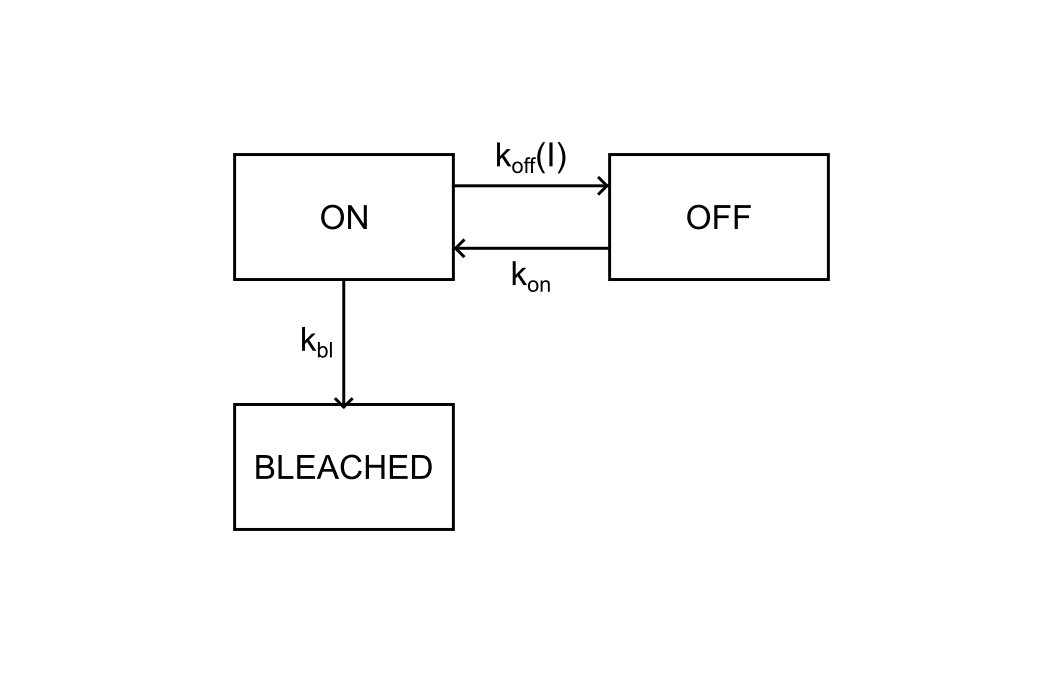
\includegraphics{three-state-photoswitching-model.png}
    \caption{Three state model of fluorescence photoswitching. Rate coefficients between states are denoted by $k$'s. $k_{off}$ is a function of light irradiance at the fluorophore. Photons are emitted from the fluorophore when it is in the ON state, but not when it is in the OFF state or the BLEACHED state. Once bleached, a fluorophore will remain that way forever.}
    \label{fig:three-state-photoswitching}
\end{figure}

At any moment in time, the fluorophore has a probability to transition to a new state that is determined only by its current state, and not by its history of transitions. This type of probabilistic model is called a Markov chain. More precisely, a fluorophore is a continuous time Markov chain because the transitions may occur at any time rather than only at discrete intervals.

Let $N$ represent the number of possible states in a Markov chain. The transitions between states are modeled as 3-tuples $\left(S_{i}, S'_{i}, t_i)\right)$, where $S \in \{ 1, \ldots, N \} $ is an integer identifying the original state of transition $i$, $S'_{i}$ is the next state, and $t_i$ is the time at which the transition occurred. Note that $S'_{i} = S_{i + 1}$. Then the set of 3-tuples $\{\ \left(S_{0}, S'_{0}, t_0)\right), \left(S_{1}, S'_{1}, t_{1})\right), \cdots \}$ describes the trajectory of the fluorophore through its energetic states over time.

Markov chains are memoryless, which means that the time to transition to the next state is independent of the time it has spent in the current state. We can model this by writing the time to transition from state $S$ to state $S'$ as an exponentially-distributed random variable\footnote{An exponential random variable models the time \textit{between} independent events. A Poisson random variable models the number of independent events during a given time.} with a probability density

\begin{equation}
    P \left(t \given S, S' \right) = k_{ \left( S, S' \right)} \exp \left( -k_{ \left( S, S' \right) } t \right)
\end{equation}

\noindent where $k_{ \left( S, S' \right)}$ is the rate coefficient from state $S$ to $S'$. When multiple states are accessible from $S$, then the transition time is still an exponentially distributed random variable. The rate coefficient to leave $S$ in this case is the sum of the rate coefficients to all the individual states, or

\begin{equation}
    k_S = \sum_{i = 1}^N k_{ \left( S, i \right) }
\end{equation}

\noindent Inaccessible states have rate coefficients of zero. So $k_{\left( \text{BLEACHED}, S' \right)} = 0$ for all $S'$.

Finally, the probability to transition to a state $S'$ from a state $S$ is given by the ratio of the rate coefficient $k_{ \left( S, S'\right)}$ to the sum of all rate coefficients from state $S$, or

\begin{equation}
    P \left(S' \given S \right) = \frac{k_{\left( S, S' \right)}}{\sum_{i = 1}^N k_{ \left( S, i \right) }}
\end{equation}

\noindent This probability may be interpreted as the probability of success in a Bernoulli trial, where success means going from state $S$ to $S'$ and failure means going from state $S$ to any other state.

Returning to \autoref{fig:three-state-photoswitching}, we can see that the rate coefficient from the ON to the OFF state depends on the laser irradiance\footnote{The units of irradiance are $W / cm^2$, or optical power per area} at visible wavelengths $I_{VIS}$. This means that increasing the laser's output power increases the rate of transitioning from the fluorescent ON state to the OFF state. Once in the OFF state, there is a small probability for the molecule to randomly return to the ON state. Additionally, we can illuminate the molecule with UV light to increase the return rate to the ON state. We can therefore balance the relative number of molecules in the ON state to the OFF state by tuning the laser irradiance in visible and UV wavelengths. This is how we achieve isolated single molecules that can be localized.

\subsection{Photoswitching vs Photoactivation}

The mechanism for ON/OFF switching that is illustrated in \autoref{fig:three-state-photoswitching} is known as \textbf{photoswitching} because fluorophores are switched between ON and OFF states using light. Photoswitching is the mechanism used in STORM to tune the density of fluorophores so that they may be localized. PALM however uses a different mechanism: \textbf{photoactivation}.

A simplified model of photoactivation is shown in \autoref{fig:four-state-photoactivation}. Here, a pulse of low-irradiance UV light illuminates a set of fluorophores within the field-of-view of the microscope. This will randomly activate a sparse subset of the fluorophores such that they can absorb light at a longer, visible wavelength. The absorbed energy is then re-emitted as fluorescence, and we can localize the fluorophore in the way we have discussed above.

\begin{figure}[ht]
    \centering
    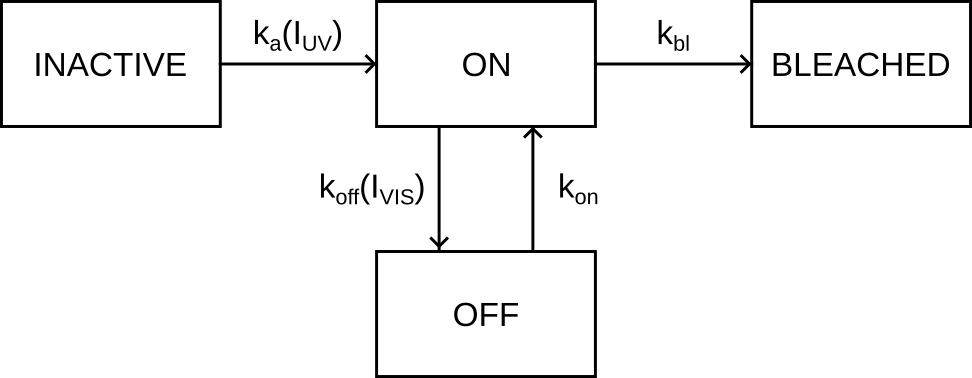
\includegraphics{four-state-photoactivation-model.png}
    \caption{Four state model of fluorescence photoactivation. Rate coefficients between states are denoted by $k$'s. $k_a$, the activation rate, is a function of light irradiance at the fluorophore in the UV part of the spectrum; $k_{off}$ is a function of irradiance in the visible part of the spectrum. Photons are emitted from the fluorophore when it is in the ON state, but not when it is in the INACTIVE, OFF, or the BLEACHED states. Once bleached, a fluorophore will remain that way forever.}
    \label{fig:four-state-photoactivation}
\end{figure}

The qualities of photoswitching and photoactivation are compared in \autoref{table:photophysics-comparison}. It's important to keep in mind that this comparison is approximate, and many exceptions can be found to it in practice.

\begin{table}
    \centering
    \begin{tabular}{ |p{4cm}|c|c| } 
        \hline
        & Photoswitching & Photoactivation \\
        \hline 
        SMLM Technique & STORM & PALM \\
        \hline
        Most common type of fluorophore & Synthetic dye & Fluorescent protein \\
        \hline
        Order of magnitude of number of photons per fluorophore per image & $10^2$ -- $10^5$ & $10^2$ -- $10^3$ \\
        \hline
        Live cell compatible & Mostly no & Mostly yes \\
        \hline
    \end{tabular}
    \caption{An approximate comparison of the qualities of the photoswitching and photoactivation mechanisms used to achieve sparse subsets of emitters in SMLM.}
    \label{table:photophysics-comparison}
\end{table}

\bibliographystyle{plain}
\bibliography{refs}

\end{document}
